\documentclass[
	article,			% article académique
	11pt,				% taille de la police
	oneside,			% impression imprimante
	a4paper,			% taille du paper
	chapter=TITLE,
	french,			% langue
	sumario=tradicional
	]{base_nt}

\usepackage{comment}

\usepackage{titlesec}
\usepackage{titletoc}

\usepackage{pgfgantt}
\usepackage{xcolor}

\definecolor{myforestgreen}{RGB}{40, 167, 69}
\definecolor{myred}{RGB}{220, 53, 69}

% Redéfinit le style des \part pour supprimer les pages générées
\titleclass{\part}{top} % Utilise le style de section "top" pour les parties
% Modifie l'espacement avant le titre de la partie
\titlespacing*{\part}{0pt}{0pt}{0pt}

\titleformat{\part}[display]{\Huge}{}{-2cm}{}

% commande simple pour afficher les commandes Latex sous forme de texte
\newcommand{\comando}[1]{\textbf{$\backslash$#1}}

\titulo{Soutenance 2 - Rapport sur le projet}

\tituloestrangeiro{Projet par des étudiants de l'EPITA}

\autor{
Félix, Yanis, Hamza, Antoine et Keany Vy \thanks{Ce rapport a été élaboré dans le cadre d'un projet réalisé à l'EPITA - (École Pour l'Informatique et les Techniques Avancées) \url{epita.fr}} 
\\[0.5cm]
\href{mailto:keany-vy.khun@epita.fr}{keany-vy.khun@epita.fr}, \href{mailto:antoine.mulot@epita.fr}{antoine.mulot@epita.fr}
\\[0.5cm]
\href{mailto:felix.despretz@epita.fr}{felix.despretz@epita.fr}, \href{ mailto:yanis.jerjini@epita.fr}{yanis.jerjini@epita.fr}, \href{mailto:hamza.khamchane@epita.fr}{hamza.khamchane@epita.fr}
\\[0.3cm]
20 juin, 2024 }


\evento{EPITA Projet S2 - Promo 2028 - Studio NeedTime()} % Bandeau au dessus de toutes les pages
\local{France}
\data{Version 1.0.1 - prod}

\begin{document}

\selectlanguage{french}

\frenchspacing 

% ----------------------------------------------------------
% ELEMENTOS PRÉ-TEXTUAIS
% ----------------------------------------------------------

%---
%
% Se desejar escrever o artigo em duas colunas, descomente a linha abaixo
% e a linha com o texto ``FIM DE ARTIGO EM DUAS COLUNAS''.
% \twocolumn[    		% INICIO DE ARTIGO EM DUAS COLUNAS
%
%---
\maketitle

\newpage
\vspace{0cm}
\begin{figure}[ht]
	\caption{Storytelling du jeu}
	\centering
	\includegraphics[width=1\linewidth]{paper1.png}
	\legend{Site web: \url{https://needtime.pages.dev/}}
	
\end{figure}

Ce rapport détaille les progrès réalisés jusqu'à présent dans le développement du jeu, ainsi que la documentation technique associée. Notre équipe a travaillé pour intégrer diverses technologies et services afin de créer un jeu innovant, unique et performant.

\vspace{0cm}
\begin{figure}[ht]
	\caption{Avancement du jeu | Soutenance 1}
	\centering
	\includegraphics[width=1\linewidth]{paper2.png}
	\legend{Site web: \url{https://needtime.pages.dev/developpement}}
	
\end{figure}

Soutenannce 1 : Le projet avance à un rythme soutenu, avec plusieurs fonctionnalités clés déjà intégrées et opérationnelles. Les phases restantes, notamment la conception des personnages et l'intelligence artificielle, sont en cours de développement et contribueront à enrichir davantage l'expérience de jeu globale. L'équipe reste engagée à respecter les délais et les normes de qualité établis, tout en s'efforçant de créer un jeu multijoueur captivant et divertissant.

\vspace{0cm}
\begin{figure}[ht]
	\caption{Avancement du jeu | Soutenance 2}
	\centering
	\includegraphics[width=1\linewidth]{paper8.png}
	\legend{Site web: \url{https://needtime.pages.dev/developpement}}
	
\end{figure}

Soutenance 2 : Le projet est désormais entièrement finalisé, avec toutes les fonctionnalités intégrées et pleinement opérationnelles. La conception des personnages et l'intelligence artificielle ont été complétées avec succès, apportan un plus à l'expérience de jeu globale. L'équipe a respecté les délais et les normes de qualité établis, créant ainsi un jeu multijoueur captivant et divertissant. Nous sommes fiers de présenter un produit finalisé qui répond aux attentes et aux standards de qualité que nous nous étions fixés.

% ----------------------------------------------------------
% ELEMENTOS TEXTUAIS
% ----------------------------------------------------------
\textual

\newpage

\customtableofcontents

% ----------------------------------------------------------
% Introduction
% ----------------------------------------------------------
%\begin{comment}
\newpage

\part{Introduction}
\section{Fonctionnalités implémentées}

\subsection{Multijoueur v1.0 - Soutenance 1}

Dans le cadre de notre projet de développement de jeu multijoueur, nous avons entrepris une création complète from scratch du système de déplacement en optant pour une solution basée sur des sockets TCP/IP en utilisant le langage C\#. Cette décision a été motivée par la volonté de créer un système original, optimisé et qui ne dépends pas de librairies ou d'APIs externes.

Nous avons opté pour des sockets TCP/IP pour la communication entre les clients et le serveur. Cette technologie offre une connexion fiable et bidirectionnelle, idéale pour un environnement multijoueur en temps réel.

Le serveur écoute en permanence les connexions entrantes des clients, acceptant les demandes de connexion et établissant des canaux de communication individuels pour chaque client.

Pour optimiser les échanges de données, nous avons mis en place un système d'écriture dans des buffers de 1 Ko. Cela permet de regrouper les données à envoyer en paquets de taille fixe, réduisant ainsi le nombre de transactions réseau et améliorant les performances globales.

Le système de transmission des données est conçu pour envoyer en continu les coordonnées des joueurs, ainsi que leurs identifiants, de manière similaire à un système de chat. Ces informations sont encapsulées dans des messages structurés, puis envoyées via les sockets aux clients concernés.

Le serveur et les clients sont équipés de mécanismes de lecture et de traitement des paquets entrants et sortants. Les données reçues sont décodées et interprétées de manière appropriée, tandis que les données à envoyer sont encapsulées dans des paquets conformes au protocole défini.

\newpage

\subsection{Multijoueur v2.0 - Soutenance 2}

Pour optimiser notre système multijoueur, nous avons décidé de passer d'une solution faite from scratch à une nouvelle architecture basée sur SpacetimeDB (logiciel open-source en Rust). Cette décision a été motivée par notre désir d'améliorer les performances, la fiabilité et l'optimisation globale de notre jeu multijoueur.

Dans la version précédente, nous avions développé un système de déplacement basé sur des sockets TCP/IP en C\# ce qui limitait le nombre de joueurs à 65535 (nombre de ports sur une machine). Cette approche nous avait permis de créer un système original et optimisé sans dépendre de bibliothèques ou d'APIs externes mais elle n'étais pas suffisante pour la version finale.

Pour la nouvelle version de notre multijoueur, nous avons donc adopté SpacetimeDB, la solution combine une base de donnée relationnelle et un serveur. Nous avons fait une intégration en C\# côté client et également en C\# côté serveur dans notre jeu. Cette architecture nous permet de connecter directement les clients à la base de donnée, exécutant ainsi la logique du jeu au sein d'une base de données locale et côté serveur. Ainsi voici les avantages et caractéristiques de la nouvelle version du multijoueur :

\begin{itemize}
    \item Architecture simplifiée : En éliminant le besoin d'un serveur intermédiaire, la communication entre les clients et la base de données est directe et plus efficace.
    \item Exécution de la logique : Les clients peuvent exécuter directement la logique du jeu dans SpacetimeDB, ce qui simplifie le code et améliore les performances.
    \item Scalabilité : La nouvelle architecture permet une meilleure gestion de la charge et une connexion plus stable pour accueillir un plus grand nombre de joueurs simultanés.
    \item Sécurité du jeu : En centralisant la logique du jeu et les données dans SpacetimeDB, nous avons pu renforcer la sécurité des échanges et empêcher la triche par utilisation d'un proxy.
\end{itemize}

\newpage

\subsection{Amélioration de l'expérience multijoueur}

\begin{itemize}
    \item Création de lobby : Permet aux joueurs de créer des espaces privés pour jouer avec leurs amis.
    \item Choisir un pseudo : Les joueurs peuvent désormais choisir et afficher leur propre pseudo en jeu.
    \item Rejoindre un lobby par son nom : Simplifie le processus de connexion entre amis.
    \item Commandes de lobby (kick, etc.) : Les hôtes peuvent gérer leur lobby de manière plus efficace.
    \item Nombre de places limitées : Contrôle du nombre de joueurs par lobby pour une meilleure gestion des ressources.
\end{itemize}

\subsection{Implémentation en C\# de la synchronisation}

\begin{itemize}
    \item Animations : Synchronisation des animations entre les clients pour une expérience cohérente.
    \item Items : Les objets sont synchronisés en temps réel entre les joueurs.
    \item Entités : Synchronisation des entités pour une interaction fluide et sans décalage.
    \item Radio : Ajout de la synchronisation de la radio pour que tous les joueurs partagent le même état de l'objet.
\end{itemize}

La radio est un élément essentiel qui participe au lore du jeu et qui a été pensé avant la conception, c'est elle qui permet aux joueurs de préparer leur échappatoire et qui représente la finalité du jeu.

\newpage

\subsection{Génération de la carte}

La génération de la carte dans notre jeu a été réalisée de manière semi-manuelle, en utilisant des outils spécifiques pour créer un environnement détaillé et réaliste. Voici comment nous avons abordé cette étape :

Création manuelle de la carte :

\begin{itemize}
    \item Plutôt que de générer la carte de manière procédurale, nous avons opté pour une approche manuelle. Cela nous a permis d'avoir un contrôle précis sur l'apparence et la disposition des éléments de la carte.
    \item Nous avons utilisé l'add-on Terrain 3D pour concevoir le relief et la topographie de la carte. Cette méthode nous a donné la possibilité de sculpter le terrain selon nos besoins, en créant des montagnes, des vallées, des plateaux, etc., de manière intuitive et personnalisée.
\end{itemize}

Utilisation de Proton Scatter pour la flore :

\begin{itemize}
    \item Pour ajouter de la végétation et des éléments naturels à la carte, nous avons intégré l'addon Proton Scatter. Cet outil nous a permis de générer aléatoirement des arbres, des arbustes, des plantes, etc., à différents endroits de la carte, créant ainsi un environnement riche et diversifié.
    \item L'utilisation de Proton Scatter nous a offert une manière efficace et réaliste d'ajouter de la flore à notre monde, en reproduisant de manière crédible les motifs de distribution des plantes dans la nature.
\end{itemize}

Génération de l'océan avec des bruits de Perlin :

\begin{itemize}
    \item Les bruits de Perlin ont été employés spécifiquement pour la génération de l'océan dans notre carte. Cette technique nous a permis de simuler les vagues et les mouvements de l'eau de manière réaliste, en créant des variations subtiles dans la texture et la hauteur de l'océan.
    \item En utilisant les bruits de Perlin, nous avons pu donner à l'océan un aspect naturel et dynamique, avec des vagues qui se déplacent de manière fluide et organique.
\end{itemize}

\subsection{Modélisation 3D}

\begin{figure}[ht]
	\caption{Modèle 3D (1)}
	\centering
	\includegraphics[width=1\linewidth]{paper7.png}
	\legend{}
	
\end{figure}

Dans notre projet, nous avons choisi de concevoir tous les modèles 3D à la main, en utilisant uniquement Blender comme outil de modélisation. Cette approche nous permet de maintenir un contrôle total sur le processus de création des modèles et de limiter notre dépendance à l'égard d'add-ons ou de logiciels tiers. En privilégiant cette méthode, nous pouvons garantir une cohérence artistique et technique dans l'ensemble de notre jeu, tout en mettant l'accent sur la qualité et l'authenticité des modèles.

L'objectif principal de notre démarche est de conserver un maximum d'authenticité dans notre jeu pour offrir une immersion optimale aux joueurs. Pour ce faire, la plupart de nos modèles sont basés sur des références et des contraintes techniques de modèles existants. Par exemple, le bombardier qui constitue la zone de départ des joueurs est largement inspiré du Boeing B-17G modèle 1941, avec la section cockpit de la version B-17E. De plus, le choix des coloris s'inspire du bombardier B-17E Shoo Shoo Shoo Baby de l'US Air Force, ajoutant ainsi une touche d'authenticité historique à notre jeu.

\begin{figure}[ht]
	\caption{Modèle 3D (2)}
	\centering
	\includegraphics[width=1\linewidth]{paper5.png}
	\legend{}
	
\end{figure}
\begin{figure}[ht]
	\caption{Modèle 3D (3)}
	\centering
	\includegraphics[width=1\linewidth]{paper6.png}
	\legend{}
	
\end{figure}

\newpage

Pour la deuxième soutenance, la modélisation 3D de notre jeu a bénéficié d'améliorations significatives pour enrichir l'expérience visuelle et immerger davantage les joueurs dans l'univers que nous avons créé. Ces améliorations ne se sont pas contentées de simplement embellir le jeu, mais ont également visé à renforcer la cohérence et la profondeur de son esthétique.

\begin{figure}[ht]
	\caption{Modèle 3D animé - Crash de l'avion}
	\centering
	\includegraphics[width=1\linewidth]{paper20.png}
	\legend{}
	
\end{figure}

En plus des améliorations des personnages et de leurs actions, nous avons également intégré un modèle d'avion qui s'est crashé, complété par des particules de flammes pour ajouter un effet spectaculaire et dramatique. Le crash de l'avion est animé de manière à montrer la destruction progressive, avec des morceaux de débris qui se détachent et tombent. Les particules de flammes ajoutent une touche de réalisme, rendant la scène encore plus immersive.

\newpage

\begin{figure}[ht]
	\caption{Modèle 3D - Rodheur}
	\centering
	\includegraphics[width=1\linewidth]{paper19.png}
	\legend{}
	
\end{figure}

Un des ajouts majeurs dans ce domaine est le nouveau modèle du joueur. Nous avons entrepris une refonte complète de ce modèle, le rendant plus détaillé et réaliste. Le nouveau modèle intègre des textures haute résolution et des animations plus fluides, ce qui contribue à un rendu visuel beaucoup plus attractif. En affinant les détails et en ajoutant des nuances réalistes, nous avons pu créer un personnage qui non seulement s'intègre harmonieusement dans l'environnement du jeu, mais qui aussi renforce l'engagement des joueurs par son aspect authentique.

\newpage

\begin{figure}[ht]
	\caption{Modèle 3D - Personnage (1)}
	\centering
	\includegraphics[width=1\linewidth]{paper17.png}
	\legend{}
	
\end{figure}

Les améliorations apportées au modèle du joueur incluent également une meilleure articulation des mouvements. Nous avons mis en place des systèmes d'animation avancés qui permettent des gestes plus naturels et crédibles. Que ce soit pour les actions de combat, les déplacements ou les interactions avec l'environnement, chaque mouvement a été soigneusement conçu pour offrir une sensation de fluidité et de réalisme. Ces ajustements améliorent considérablement l'immersion et rendent l'expérience de jeu plus captivante.

\newpage

\begin{figure}[ht]
	\caption{Modèle 3D - Hache}
	\centering
	\includegraphics[width=1\linewidth]{paper18.png}
	\legend{}
	
\end{figure}

En plus du modèle du joueur, l'environnement 3D du jeu a également été enrichi avec des éléments plus complexes et diversifiés. Les textures des décors ont été affinées, les effets d'éclairage retravaillés et les objets du décor détaillés avec une précision supérieure.

\newpage

\subsection{Animations}

Dans notre projet, nous avons apporté une attention particulière aux animations des personnages pour garantir une expérience de jeu immersive et fluide. Les animations du Prowler (rodeur) ont été réalisées manuellement sur Blender, un logiciel de modélisation 3D, puis exportées dans Godot. Cette approche nous a permis d'avoir un contrôle total sur le processus de création des animations, nous assurant ainsi qu'elles correspondent parfaitement à nos besoins et à l'esthétique de notre jeu.

\begin{figure}[ht]
	\caption{AnimationTree Node du Player - Soutenance 1}
	\centering
	\includegraphics[width=1\linewidth]{paper4.png}
	\legend{}
	
\end{figure}

Quant aux animations du personnage joueur, nous avons utilisé l'outil en ligne de rigging et d'animation de personnages d'Adobe, appelé Mixamo. Nous avons importé les animations de Mixamo dans Blender pour les modifier et les harmoniser avec l'armature du personnage. Cette étape était essentielle pour garantir la cohérence visuelle et le réalisme des mouvements du personnage. Une fois les animations ajustées dans Blender, nous les avons exportées dans Godot.

\begin{figure}[ht]
	\caption{AnimationTree Node du Player - Soutenance 2}
	\centering
	\includegraphics[width=1\linewidth]{paper22.png}
	\legend{}
	
\end{figure}

\newpage

Dans Godot, nous avons connecté notre modèle de personnage et ses animations à un noeud AnimationTree. Ce noeud nous a permis d'organiser les animations et de les déclencher en fonction de conditions spécifiques, telles que des booléens. Cette approche nous a donné un contrôle précis sur le déroulement des animations dans le jeu, nous permettant d'offrir une expérience de jeu dynamique et immersive pour les joueurs.

\newpage

Pour la deuxième soutenance, les animations de notre jeu ont été largement améliorées pour offrir une expérience visuelle plus immersive et captivante. Ces améliorations visent à enrichir la dynamique du jeu, rendant chaque interaction plus engageante et réaliste pour les joueurs.

\begin{figure}[ht]
	\caption{Modèle 3D animé - Radio réparée}
	\centering
	\includegraphics[width=1\linewidth]{paper15.png}
	\legend{}
	
\end{figure}

Une des principales améliorations réside dans l'augmentation du nombre d'animations disponibles. Nous avons doublé le nombre d'animations par rapport à la version précédente, ce qui permet une plus grande variété dans les mouvements des personnages. Cette diversité ajoute de la richesse à l'expérience de jeu, en offrant des animations spécifiques pour une multitude d'actions et de situations. Qu'il s'agisse de combats, d'explorations, ou d'interactions avec l'environnement, chaque action bénéficie maintenant de sa propre animation.

\begin{figure}[ht]
	\caption{Modèle 3D animé - Radio endommagée}
	\centering
	\includegraphics[width=1\linewidth]{paper14.png}
	\legend{}
	
\end{figure}

\newpage

En parallèle de l'augmentation du nombre d'animations, chaque animation a été retravaillée pour offrir plus de précision et de réalisme. Les mouvements ont été affinés pour paraître plus naturels, avec une attention particulière portée aux détails tels que les transitions entre les actions et les réponses aux interactions de l'utilisateur. Cette attention au détail permet de créer des personnages dont les gestes sont non seulement cohérents avec leur apparence mais aussi avec leur environnement et les situations qu'ils rencontrent.

\newpage

\begin{figure}[ht]
	\caption{Modèle 3D animé - Personnage (2)}
	\centering
	\includegraphics[width=1\linewidth]{paper16.png}
	\legend{}
	
\end{figure}

Les animations de combat, par exemple, intègrent maintenant des enchaînements plus fluides et des impacts plus percutants, donnant aux affrontements une dimension plus dynamique et intense. Les animations de déplacement ont été améliorées pour inclure des variations subtiles en fonction du terrain et de la vitesse.

\newpage

\vspace{0cm}

\subsection{Interactions joueurs / carte}


La gestion des interactions entre les joueurs et le Terrain3D, en tenant compte des collisions pour assurer un gameplay fluide et réaliste. Voici comment nous avons mis en place cette fonctionnalité :

\begin{itemize}
    \item Utilisation des collisions: Nous avons intégré des collisions entre les objets du jeu, y compris les joueurs et le Terrain3D. Godot Engine propose un système de collisions robuste qui permet de détecter les collisions entre les objets, ainsi que de gérer les réponses appropriées, comme la détection de contact, la résolution de collisions et la restitution des interactions.
    \item Optimisation des performances: Pour garantir des performances fluides, en particulier dans les jeux en monde ouvert où de nombreux éléments du Terrain3D peuvent être présents, nous avons optimisé la gestion des collisions. Cela peut inclure la mise en place de systèmes de partitionnement spatial pour limiter le nombre de collisions vérifiées à chaque frame, ou l'utilisation de modèles de collision simplifiés pour les objets complexes.
\end{itemize}

Les interactions entre les joueurs et la carte ont été enrichies par l'ajout de nouvelles fonctionnalités et la refonte de systèmes existants :

\begin{itemize}
    \item Refonte du système d'inventaire : Une nouvelle interface et une meilleure gestion des objets.
    \item Implémentation de la radio à réparer : Ajout d'un nouvel élément interactif qui ajoute de la profondeur au gameplay.
    \item Système de stockage (coffres) : Permet aux joueurs de stocker et de gérer leurs items de manière organisée.
\end{itemize}

\newpage

\subsection{Implémentation jouabilité}

Voici comment nous avons abordé cette étape dans notre projet :

\begin{itemize}
    \item Définition des mécaniques de jeu : Avant de commencer l'implémentation, nous avons défini clairement les mécaniques de jeu que nous souhaitions inclure. Cela inclut les actions que les joueurs peuvent effectuer, les objectifs à atteindre, les règles du jeu, etc.
    \item Prototypage et itérations : Nous avons commencé par créer des prototypes simples pour tester nos idées de jeu et itérer rapidement sur celles-ci. Les prototypes nous ont permis d'identifier ce qui fonctionne bien et ce qui doit être amélioré, et nous ont aidés à affiner nos mécaniques de jeu avant de passer à l'implémentation complète.
    \item Implémentation des contrôles : Nous avons mis en place les contrôles du jeu, y compris les interactions joueur/clavier ou manette. Nous avons veillé à ce que les contrôles soient intuitifs et réactifs, offrant ainsi aux joueurs une expérience de jeu fluide et agréable.
    \item Intégration des mécaniques de jeu : Nous avons ensuite implémenté les différentes mécaniques de jeu, telles que l'épuisement, l'exploration, la collecte d'objets, etc. Chaque mécanique a été soigneusement conçue pour offrir une expérience de jeu diversifiée et captivante.
    \item Équilibrage du gameplay : L'équilibrage du gameplay est essentiel pour garantir une expérience de jeu juste et gratifiante. Nous avons ajusté les paramètres du jeu, tels que le déplacement des personnages, l'épuisement et l'intéraction avec les objets.
\end{itemize}

\newpage

Pour la deuxième soutenance, la jouabilité de notre jeu a été significativement renforcée grâce à l'ajout de nouvelles fonctionnalités et à l'amélioration globale de l'expérience utilisateur.

\begin{figure}[ht]
	\caption{Tutoriel Jeu (1)}
	\centering
	\includegraphics[width=1\linewidth]{paper23.png}
	\legend{}
	
\end{figure}

\begin{figure}[ht]
	\caption{Tutoriel Jeu (2)}
	\centering
	\includegraphics[width=1\linewidth]{paper24.png}
	\legend{}
	
\end{figure}

\newpage

Une des principales améliorations apportées concerne l'introduction de plusieurs nouveaux items. Ces objets, variés et nombreux, ont été soigneusement conçus pour enrichir le gameplay. Chaque item apporte de nouvelles possibilités stratégiques et tactiques, encourageant les joueurs à explorer différentes approches et styles de jeu. Qu'il s'agisse d'armes, d'outils, ou d'objets utilitaires, chaque nouvel ajout a été pensé pour offrir des avantages spécifiques et des défis uniques, augmentant ainsi la profondeur et la complexité du jeu. Ces items variés permettent aux joueurs de personnaliser leur expérience, rendant chaque partie unique et engageante.

\begin{figure}[ht]
	\caption{Tutoriel Jeu (3)}
	\centering
	\includegraphics[width=1\linewidth]{paper25.png}
	\legend{}
	
\end{figure}

\newpage

\begin{figure}[ht]
	\caption{Tutoriel Jeu (4)}
	\centering
	\includegraphics[width=1\linewidth]{paper26.png}
	\legend{}
	
\end{figure}

En complément de ces nouveaux items, nous avons également introduit un niveau de tutoriel. Ce niveau a été conçu pour guider les nouveaux joueurs à travers les mécanismes fondamentaux du jeu, leur permettant de se familiariser rapidement avec les commandes et les systèmes en place. Le tutoriel offre des explications claires et des démonstrations pratiques, aidant les joueurs à comprendre les bases du gameplay et à se sentir plus à l'aise dans l'environnement du jeu. Cette introduction progressive réduit la courbe d'apprentissage et minimise la frustration des nouveaux venus, tout en leur permettant de saisir rapidement les éléments essentiels pour une expérience de jeu réussie.

\newpage

\subsection{Sons / Effets spéciaux et IA}

Sons / Effets spéciaux :

\begin{itemize}
    \item Conception sonore : Nous avons élaboré une conception sonore détaillée pour donner vie à notre jeu. Cela comprend la création ou l'acquisition de divers effets sonores tels que les bruits de pas, les tirs d'armes, les explosions, les ambiances environnementales, etc.
    \item Effets visuels : Nous avons également travaillé sur les effets visuels pour rendre le jeu plus immersif. Cela comprend l'animation des personnages et des objets, les effets du soleil, les jeux de lumière, etc. Ces éléments contribuent à créer un monde virtuel vivant et vibrant.
\end{itemize}

Intelligence Artificielle (IA) :

\begin{itemize}
    \item Prise de décision : L'IA est capable de suivre le joueur en temps réel en fonction de divers facteurs tels que la position des joueurs, les objectifs, etc. Cela permet aux personnages de s'adapter aux situations changeantes et de fournir un défi continu aux joueurs.
\end{itemize}

\vspace{2.3cm}

\newpage

\vspace*{5cm}

\part{Problèmes rencontrés}
\section{Résolution des problèmes}

\subsection{Bugs et obsolescence}

Au cours du développement, nous avons fait face à des défis liés à l'implémentation de l'API 4 de Godot, ce qui a nécessité une réévaluation de notre approche pour la fonctionnalité multijoueur. Voici un aperçu des problèmes rencontrés et des solutions que nous avons adoptées :

\begin{itemize}
    \item Implémentation de l'API 4 de Godot : Nous avons initialement envisagé d'utiliser l'API 4 de Godot pour gérer le multijoueur de notre jeu. Cependant, nous avons rencontré des difficultés techniques avec cette version, notamment des incompatibilités avec certaines librairies que nous avions l'intention d'utiliser.
    \item Construction du Système : Face à ces défis, nous avons pris la décision de construire notre propre système multijoueur à partir de zéro, en utilisant des sockets TCP/IP en langage C\#. Cette approche nous a offert un plus grand contrôle sur la communication réseau et nous a permis de contourner les problèmes rencontrés avec l'API 4 de Godot.
    \item Éviter les Dépendances Inutiles : Une autre complication était la version relativement récente de Godot par rapport à certaines librairies tierces que nous avions l'intention d'utiliser. Pour éviter les problèmes de compatibilité et les obsolescences potentielles, nous avons décidé de minimiser notre dépendance à ces librairies, en nous concentrant sur des solutions internes autant que possible.
\end{itemize}

\newpage

\subsection{Merge conflicts et versions}

Pendant le développement de notre projet, nous avons été confrontés à des défis liés aux différentes versions de Godot utilisées par les membres de notre équipe, ainsi qu'aux variations des systèmes d'exploitation. Voici comment nous avons abordé ces problèmes :

\begin{itemize}
    \item Variations des Versions de Godot : En raison des différentes versions de Godot utilisées par les membres de notre équipe, nous avons rencontré des situations où le code développé sur une version spécifique de Godot ne fonctionnait pas correctement sur d'autres versions. Cela a entraîné des conflits de fusion lors de l'intégration du code dans le référentiel commun.
    \item Diversité des Systèmes d'Exploitation : Notre équipe travaillait sur différents systèmes d'exploitation, ce qui a ajouté une autre couche de complexité à la gestion des versions. Les différences dans la configuration et le comportement des systèmes ont parfois entraîné des incohérences dans le code et des problèmes de compatibilité.
    \item Communication et Coordination : Pour surmonter ces défis, nous avons dû mettre en place des pratiques de gestion de version rigoureuses. Cela comprenait l'utilisation de rebases pour réorganiser l'historique des commits, des reverts pour annuler les modifications indésirables, et des résolutions de merge conflicts pour harmoniser les différences entre les branches.
\end{itemize}

Nous avons également adopté une approche proactive en mettant en place un fichier .gitignore pour ignorer les fichiers temporaires et les artefacts de build générés par Godot. Cela nous a permis de maintenir un référentiel propre et de minimiser les conflits liés aux fichiers inutiles.

\part{Conception et from scratch}

\section{Design patterns (UML)}

Pour concevoir notre architecture logicielle, nous avons opté pour l'utilisation de design patterns afin de garantir une structure modulaire, extensible et facilement maintenable. En utilisant le langage UML (Unified Modeling Language), nous avons représenté nos design patterns à travers des diagrammes de classes, de séquence et d'états, selon les besoins spécifiques de chaque composant du système.

Multiplayer.cs (Soutenance 1)

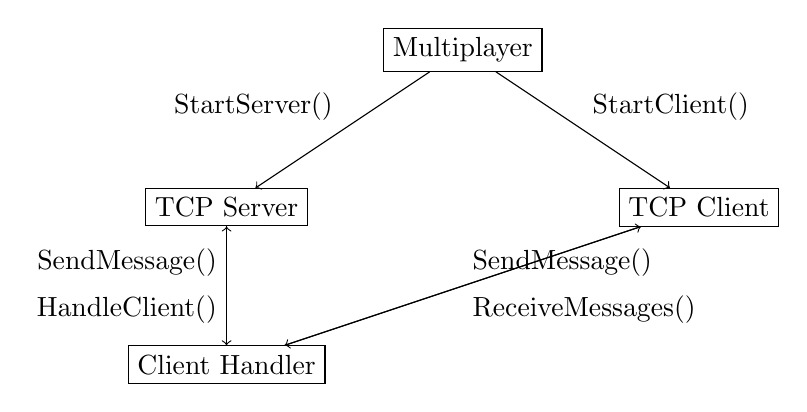
\begin{tikzpicture}[node distance=2cm]

% Nodes
\node (multiplayer) [rectangle, draw] {Multiplayer};
\node (tcpserver) [rectangle, draw, below of=multiplayer, xshift=-3cm] {TCP Server};
\node (tcpclient) [rectangle, draw, below of=multiplayer, xshift=3cm] {TCP Client};
\node (clienthandler) [rectangle, draw, below of=tcpserver] {Client Handler};

% Arrows
\draw[->] (multiplayer) -- node[above left] {StartServer()} (tcpserver);
\draw[->] (multiplayer) -- node[above right] {StartClient()} (tcpclient);
\draw[->] (tcpserver) -- node[below left] {HandleClient()} (clienthandler);
\draw[->] (tcpclient) -- node[below right] {ReceiveMessages()} (clienthandler);
\draw[->] (clienthandler) -- node[above left] {SendMessage()} (tcpserver);
\draw[->] (clienthandler) -- node[above right] {SendMessage()} (tcpclient);

\end{tikzpicture}

\section{Optimisations et réflexions}

\subsection{Mécaniques spécifiques}

Barre de Stamina :

\begin{itemize}
    \item Fonctionnement : La barre de stamina est une ressource limitée qui se vide lorsque le joueur effectue des actions gourmandes en énergie, telles que la course, les sauts ou les attaques puissantes. Elle se recharge progressivement lorsque le joueur se repose ou adopte un rythme plus lent.
    \item Impact sur le gameplay : La gestion de la stamina est cruciale pour la survie et la réussite dans le jeu. Un joueur épuisé sera moins efficace dans le combat et la traversée de l'environnement. Cela encourage les joueurs à adopter des stratégies tactiques, à planifier leurs mouvements et à prendre des décisions réfléchies pour optimiser l'utilisation de leur énergie.
\end{itemize}

Inventaire du joueur :

\begin{itemize}
    \item Gestion des objets : Le joueur dispose d'un inventaire dans lequel il peut transporter une variété d'objets, tels que des armes, des outils, des consommables, etc. Chaque objet occupe un certain nombre de slots dans l'inventaire, limitant la quantité d'objets qu'un joueur peut transporter simultanément.
    \item Interaction avec les objets : Le joueur peut interagir avec les objets de son inventaire, en les utilisant pour différentes actions telles que l'attaque, la défense, la guérison, etc. De plus, le joueur a la possibilité de jeter des objets de son inventaire pour libérer de l'espace ou pour les utiliser comme projectiles.
    \item Ramassage d'objets : Les joueurs peuvent ramasser des objets dispersés dans l'environnement en les approchant et en appuyant sur une touche dédiée. Cela permet de collecter des ressources, des armes, des équipements, etc., pour améliorer les capacités et les chances de survie du joueur.
\end{itemize}

\newpage

\subsection{Applications de la vie réelle}

Dans le contexte de l'application de la vie réelle, le fonctionnement du système multijoueur (Soutenance 1) repose sur le principe fondamental d'un chat serveur-client. Tout comme dans un chat en ligne où les utilisateurs envoient et reçoivent des messages, dans notre système multijoueur, nous échangeons des données de manière similaire. Cependant, au lieu d'envoyer des messages textuels, nous transmettons des données sous forme de tuples.

Chaque tuple contient deux parties principales. Le premier paramètre est l'identifiant unique du client, qui permet au serveur de distinguer et d'identifier chaque client connecté de manière unique. Le deuxième paramètre est un triplet contenant les coordonnées spatiales du client dans le monde du jeu, généralement représentées par les coordonnées x, y et z.

Ces données sont encapsulées dans une chaîne de caractères (string) avant d'être envoyées via le réseau. Lorsqu'elles sont reçues par le destinataire, elles sont analysées (parsées) pour extraire les informations pertinentes, telles que l'identifiant du client et ses coordonnées spatiales.

Ce fonctionnement basé sur le principe d'un chat serveur-client offre une solution élégante pour synchroniser les actions des différents joueurs dans le jeu. Il permet une communication efficace entre le serveur et les clients, facilitant ainsi la mise à jour et la coordination des éléments du jeu pour tous les participants.

\newpage

De plus dsans notre projet, nous avons adopté pour une approche minimaliste en ce qui concerne l'utilisation d'assets et d'add-ons externes. Notre objectif principal était de réduire au maximum les dépendances extérieures afin de maintenir un contrôle total sur le développement de notre jeu. Cette stratégie nous a permis d'optimiser les performances et de simplifier les processus de développement, de déploiement et de maintenance.

En limitant l'utilisation d'assets préfabriqués et d'add-ons tiers, nous avons également pu minimiser la complexité de notre code et améliorer son efficacité.

Cela nous a donné la possibilité de concevoir des systèmes personnalisés et d'optimiser chaque aspect de notre jeu pour offrir la meilleure expérience possible aux joueurs. En fin de compte, cette approche nous a permis de créer un jeu qui reflète pleinement notre vision créative, tout en garantissant une performance optimale et une flexibilité maximale dans le développement.

\newpage

\section{Création du launcher}

Nous avons développé un launcher en C\#, intégrant l'exécutable du jeu et tous les assets nécessaires. Le choix de C\# et .NET Framework sa compatibilité avec Windows et le jeu étant fait dans ce langage il était logique de poursuivre sur le même langage.

Le launcher inclut l'exécutable du jeu, les assets et l'icône du jeu, tous compressés avec l'algorithme LZMA (Lempel-Ziv-Markov chain algorithm) pour une réduction maximale de la taille des fichiers. 

\begin{figure}[ht]
	\caption{Lempel-Ziv-Markov chain
algorithm}
	\centering
	\includegraphics[width=1\linewidth]{paper9.png}
	\legend{}
	
\end{figure}

LZMA a l'avantage d'avoir un excellent ratio de compression et une décompression rapide (même si la compression est plus lente), optimisant ainsi l'espace de stockage et l'nstallation de notre jeu.

\newpage

\begin{figure}[ht]
	\caption{Launcher (installation)}
	\centering
	\includegraphics[width=1\linewidth]{paper10.png}
	\legend{}
	
\end{figure}

Ainsi, le processus d'installation est simplifié : l'utilisateur télécharge un unique fichier compressé (contenu dans la launcher), que le launcher décompresse rapidement grâce à l'algorithme de compression. L'installation de l'exécutable et des assets est automatisée, et les raccourcis pointant sur l'exécutable du jeu sont ajoutés au bureau et au menu démarrer.

\newpage

Le launcher détecte également si le jeu est déjà installé. En cas de détection positive, il propose des options de désinstallation ou de réparation des fichiers corrompus, facilitant ainsi la gestion et la maintenance.

\begin{figure}[ht]
	\caption{Launcher (désinstallation/réparation)}
	\centering
	\includegraphics[width=1\linewidth]{paper11.png}
	\legend{}
	
\end{figure}

Cette approche permet donc une installation plus facile et plus rapide pour l'utilisateur, tout en permetant de réduire le temps et l'espace de stockage nécessaires.

\newpage

\part{Outils et frameworks utilisés}

\section{Gestion de configuration}

\subsection{Github vs Gitlab vs Gitea}


La gestion de la configuration revêt une importance capitale dans le développement de tout projet logiciel, car elle permet de centraliser et de contrôler les différentes versions du code source. Lorsque nous avons choisi une plateforme pour héberger notre dépôt Git, nous avons pris en compte plusieurs facteurs, dont la fiabilité, la facilité d'utilisation et la popularité.

Nous avons sélectionné Github pour sa grande popularité à l'échelle mondiale, tant dans les entreprises que dans la communauté open source. Cette large adoption signifie qu'il existe une vaste base d'utilisateurs et de contributeurs potentiels, ce qui facilite la collaboration et le partage des connaissances. De plus, la familiarité avec GitHub est un avantage significatif pour de nombreux développeurs, car ils sont déjà habitués à son interface et à ses fonctionnalités.

De plus il offre une intégration transparente avec de nombreux autres outils et services couramment utilisés dans le développement logiciel, tels que des services d'intégration continue (CI/CD) comme Travis CI ou GitHub Actions, ainsi que des outils de gestion de projet comme ZenHub ou Projects. Cette intégration facilite le processus de développement en permettant une automatisation et une collaboration efficaces entre les différents aspects du cycle de vie du développement logiciel.

\newpage

\subsection{Sécurité, authenticité, backups}

Pour garantir la sécurité et l'intégrité de notre projet, nous avons mis en place plusieurs mesures de sécurité importantes au niveau de notre dépôt GitHub. Voici comment nous avons renforcé la sécurité de notre dépôt :

\begin{itemize}
    \item Vérification des clés SSH : Nous avons configuré la vérification des clés SSH pour l'accès à notre dépôt GitHub. Cela signifie que seuls les utilisateurs disposant de clés SSH valides et autorisées peuvent accéder au dépôt. Les clés SSH offrent une méthode sécurisée d'authentification des utilisateurs lors de l'accès au dépôt, ce qui renforce la sécurité de nos données.
    \item Backups automatisées : Nous avons mis en place des sauvegardes automatisées de notre dépôt GitHub pour garantir la disponibilité continue de nos données. En sauvegardant régulièrement notre dépôt, nous nous assurons que même en cas de problème technique ou de perte de données, nous disposons toujours d'une copie de sauvegarde à restaurer.
    \item Vérification des clés GPG : Nous avons également mis en place la vérification des clés GPG pour garantir l'authenticité des membres de notre équipe. Chaque membre de l'équipe dispose d'une clé GPG qui est utilisée pour signer ses contributions au dépôt. Lorsqu'une contribution est soumise, elle est vérifiée à l'aide de la clé GPG correspondante pour s'assurer qu'elle provient bien du membre de l'équipe légitime. Cela renforce la confiance dans l'authenticité des contributions et prévient toute tentative de modification non autorisée du code source.
\end{itemize}

\newpage

\section{Moteur de jeu 3D}

\subsection{Godot, C\#}

Nous avons choisi Godot comme moteur de jeu pour notre projet, principalement en raison de plusieurs avantages techniques et pratiques qu'il offre par rapport à d'autres moteurs de jeu, comme Unity, par exemple.

\begin{itemize}
    \item Open-source: Godot est un moteur de jeu open-source, ce qui signifie que son code source est accessible à tous et peut être modifié et étendu selon les besoins du projet. Cette ouverture permet une plus grande transparence et offre une flexibilité totale dans le développement.
    \item Gratuité: En tant que moteur de jeu open-source, Godot est gratuit à utiliser, ce qui réduit considérablement les coûts de développement. Cela signifie que les petites équipes ou les développeurs indépendants peuvent accéder à des outils puissants sans avoir à payer de licences coûteuses.
    \item Flexibilité du langage de script: Godot offre une flexibilité significative en matière de langage de script. Il utilise GDScript, un langage de script similaire à Python, qui est facile à apprendre et à utiliser avec du C\#. Cela permet aux développeurs de créer rapidement des prototypes et d'itérer sur le jeu avec facilité.
    \item Performance: Godot est reconnu pour sa légèreté et ses performances élevées. Son moteur de rendu optimisé et son architecture modulaire permettent d'obtenir des performances optimales, même sur des appareils moins puissants, ce qui est crucial pour garantir une expérience fluide aux joueurs.
    \item Communauté active: Godot bénéficie d'une communauté active et dévouée de développeurs, d'artistes et de contributeurs. Cette communauté fournit un soutien technique, des ressources utiles, des didacticiels et des plugins qui enrichissent l'écosystème de développement et facilitent le processus de création de jeux.
\end{itemize}

\subsection{Addons :}

\begin{itemize}
    \item Mixamo from Adobe :  \url{https://www.mixamo.com/}
    \item Terrain3D :  \url{https://github.com/TokisanGames/Terrain3D}
    \item ProtonScatter :  \url{ https://github.com/HungryProton/scatter}
\end{itemize}

\begin{figure}[ht]
	\caption{Modèle 3D - Carte}
	\centering
	\includegraphics[width=1\linewidth]{paper21.png}
	\legend{}
	
\end{figure}

\newpage

\section{Multijoueur et serveur}

\subsection{SpacetimeDB}

Pour optimiser notre système multijoueur et garantir une performance élevée ainsi qu'une sécurité renforcée, nous avons choisi d'utiliser SpacetimeDB en combinaison avec un serveur Microsoft Azure sous Linux.

\begin{figure}[ht]
	\caption{Serveur Microsoft Azure (1)}
	\centering
	\includegraphics[width=1\linewidth]{paper12.png}
	\legend{}
	
\end{figure}

\newpage

\begin{figure}[ht]
	\caption{Serveur Microsoft Azure (2)}
	\centering
	\includegraphics[width=1\linewidth]{paper28.png}
	\legend{}
	
\end{figure}

\begin{figure}[ht]
	\caption{Serveur Microsoft Azure (3)}
	\centering
	\includegraphics[width=1\linewidth]{paper29.png}
	\legend{}
	
\end{figure}

Pour héberger notre instance de SpacetimeDB, nous avons opté pour un serveur Azure. L'offre Microsoft Azure, étant utilisée en entreprise et permettant de gérer facilement les besoins croissants de notre jeu multijoueur. Le choix de Linux comme système d'exploitation pour le serveur garantit donc une utilisation efficace des ressources et une stabilité au niveau de l'uptime.

\newpage

\subsection{Docker}

Pour isoler et sécuriser notre instance de SpacetimeDB, nous l'avons déployée dans un conteneur Docker sur notre serveur Azure. L'utilisation de Docker présente plusieurs avantages :

\begin{itemize}
    \item Légèreté : Les conteneurs Docker consomment moins de ressources que les machines virtuelles traditionnelles, ce qui rend l'instance plus légère et plus rapide.
    \item Sécurité : Docker offre une couche supplémentaire de sécurité en isolant l'application du système hôte. En cas d'attaque, les intrus ne peuvent pas accéder directement à la machine hôte à partir du conteneur. (nous avons limité au maximum les permissions du container)
    \item Portabilité : Les conteneurs Docker peuvent être facilement déplacés et déployés sur d'autres serveurs ou environnements, simplifiant ainsi la gestion et la maintenance.
\end{itemize}

\begin{figure}[ht]
	\caption{Image de SpacetimeDB}
	\centering
	\includegraphics[width=1\linewidth]{paper27.png}
	\legend{}
	
\end{figure}

\newpage

\begin{figure}[ht]
	\caption{Container docker}
	\centering
	\includegraphics[width=1\linewidth]{paper13.png}
	\legend{}
	
\end{figure}

Docker nous permet également de savoir via le container si SpacetimeDB a planté et donc de mettre à jour plus facilement la configuration de l'instance.

\newpage

\section{Frameworks et hébergement}

\subsection{React, Vanilla JS, Cloudflare}

\begin{itemize}
    \item Librairies JS :  \url{https://webpack.js.org/}, \url{https://web.dev/explore/progressive-web-apps}, \url{https://lottiefiles.com}, \url{https://ogp.me}
    \item Vanilla JS : \url{https://github.com/zloirock/core-js}, \url{https://mobx.js.org}
\end{itemize}

\begin{itemize}
    \item Cloudflare : Hébergement statique et utilisation du CDN
    \item Mailchimp : Serveur SMTP, IMAP et POP3 + Cloudflare Workers
\end{itemize}

\newpage

\section{Avancement et Planification}

2024-03-20 : Nous avons atteint environ 80\% de nos objectifs initiaux pour la première soutenance de notre projet. Il nous reste encore quelques étapes à franchir pour parachever notre vision globale. Les tâches restantes comprennent l'implémentation de la carte avec des éléments tels que des grottes et de la végétation, l'ajout de plus de types de monstres pour enrichir l'expérience de jeu, le développement de designs de personnages plus complets et variés, ainsi que l'implémentation d'une version en ligne pour permettre le jeu sur le WAN en plus du LAN.

2024-06-14 : Depuis la première soutenance, nous avons fait d'énormes progrès et avons maintenant atteint tous nos objectifs initiaux. L'ensemble des fonctionnalités et des éléments prévus pour le jeu ont été entièrement implémentés et sont pleinement opérationnels. Cependant, au cours du développement, nous avons décidé de retirer certaines idées initiales pour améliorer la jouabilité. Par exemple, bien que nous avions initialement prévu de créer 4-5 personnages, nous avons réduit ce nombre et nous avions également prévu d'intégrer divers sons et effets spéciaux. Or, c'est lors des phases de test, que nous avons constaté que certains de ces éléments étaient gênants pendant les parties. Par conséquent, nous avons donc choisi de les retirer pour garantir une expérience de jeu plus fluide et agréable.

\newpage

\subsection{Tableau de planification d'avancement des tâches}

Avant la 1ère soutenance :

    \begin{center}
    \begin{ganttchart}[
        y unit title=0.4cm,
        y unit chart=0.5cm,
        vgrid,
        hgrid,
        title label anchor/.style={below=-1.6ex},
        title left shift=.05,
        title right shift=-.05,
        title height=1,
        progress label text={},
        bar height=0.7,
        group right shift=0,
        group top shift=.6,
        group height=.3,
        bar/.append style={fill=myforestgreen},
        bar/.append style={draw=black!50},
        bar incomplete/.style={fill=myred}
    ]{1}{24}
    
    % Labels
    \gantttitle{Diagramme de Gantt}{24} \\
    \gantttitle{Soutenance 22-29 janvier}{8}
    \gantttitle{Soutenance 18-22 mars}{8}
    \gantttitle{Soutenance 17-21 juin}{8} \\
    
    % Tâches
    \ganttbar[progress=15]{Site web}{1}{11} 
    \ganttbar[progress=0]{}{22}{24}\\
    \ganttbar[progress=0]{Conception des personnages}{1}{13}
    \ganttbar[progress=0]{}{23}{24}\\
    \ganttbar[progress=3]{}{1}{5}
    \ganttbar[progress=0]{Modélisation 3D}{12}{20} \\
    \ganttbar[progress=10]{Développement Lore}{1}{17}\\
    \ganttbar[progress=0]{Intereactions joueurs/carte}{3}{17}
    \ganttbar[progress=0]{}{22}{24}\\
    \ganttbar[progress=0]{Implémentation jouabilité}{5}{19}\\
    \ganttbar[progress=0]{Intelligence artificielle}{6}{20}\\
    \ganttbar[progress=0]{Animations}{7}{13}\\
    \ganttbar[progress=0]{}{1}{2}
    \ganttbar[progress=0]{Multijoueur}{9}{24} \\
    \ganttbar[progress=0]{}{1}{3}
    \ganttbar[progress=0]{Interface graphique du jeu}{14}{24}\\
    \ganttbar[progress=5]{Génération de la carte}{1}{6}
    \ganttbar[progress=0]{}{15}{24}\\
    \ganttbar[progress=0]{}{4}{8}
    \ganttbar[progress=0]{Textures / Rendu}{16}{24}\\
    \ganttbar[progress=0]{Sons / Effets spéciaux}{20}{24}
    
    \end{ganttchart}
    \end{center}

Première soutenance - dernière modifcation 2024-03-20 :
    \begin{center}
    \begin{ganttchart}[
        y unit title=0.4cm,
        y unit chart=0.5cm,
        vgrid,
        hgrid,
        title label anchor/.style={below=-1.6ex},
        title left shift=.05,
        title right shift=-.05,
        title height=1,
        progress label text={},
        bar height=0.7,
        group right shift=0,
        group top shift=.6,
        group height=.3,
        bar/.append style={fill=myforestgreen},
        bar/.append style={draw=black!50},
        bar incomplete/.style={fill=myred}
    ]{1}{24}
    
    % Labels
    \gantttitle{Diagramme de Gantt}{24} \\
    \gantttitle{Soutenance 22-29 janvier}{8}
    \gantttitle{Soutenance 18-22 mars}{8}
    \gantttitle{Soutenance 17-21 juin}{8} \\
    
    % Tâches
    \ganttbar[progress=100]{Site web}{1}{11} 
    \ganttbar[progress=0]{}{22}{24}\\
    \ganttbar[progress=60]{Conception des personnages}{1}{13}
    \ganttbar[progress=0]{}{23}{24}\\
    \ganttbar[progress=100]{}{1}{5}
    \ganttbar[progress=30]{Modélisation 3D}{12}{20} \\
    \ganttbar[progress=10]{Développement Lore}{1}{17}\\
    \ganttbar[progress=20]{Intereactions joueurs/carte}{3}{17}
    \ganttbar[progress=0]{}{22}{24}\\
    \ganttbar[progress=20]{Implémentation jouabilité}{5}{19}\\
    \ganttbar[progress=10]{Intelligence artificielle}{6}{20}\\
    \ganttbar[progress=80]{Animations}{7}{13}\\
    \ganttbar[progress=100]{}{1}{2}
    \ganttbar[progress=20]{Multijoueur}{9}{24} \\
    \ganttbar[progress=100]{}{1}{3}
    \ganttbar[progress=5]{Interface graphique du jeu}{14}{24}\\
    \ganttbar[progress=100]{Génération de la carte}{1}{6}
    \ganttbar[progress=5]{}{15}{24}\\
    \ganttbar[progress=100]{}{4}{8}
    \ganttbar[progress=0]{Textures / Rendu}{16}{24}\\
    \ganttbar[progress=0]{Sons / Effets spéciaux}{20}{24}
    
    \end{ganttchart}
    \end{center}

\newpage

Deuxième soutenance - dernière modifcation 2024-06-14 :
    \begin{center}
    \begin{ganttchart}[
        y unit title=0.4cm,
        y unit chart=0.5cm,
        vgrid,
        hgrid,
        title label anchor/.style={below=-1.6ex},
        title left shift=.05,
        title right shift=-.05,
        title height=1,
        progress label text={},
        bar height=0.7,
        group right shift=0,
        group top shift=.6,
        group height=.3,
        bar/.append style={fill=myforestgreen},
        bar/.append style={draw=black!50},
        bar incomplete/.style={fill=myred}
    ]{1}{24}
    
    % Labels
    \gantttitle{Diagramme de Gantt}{24} \\
    \gantttitle{Soutenance 22-29 janvier}{8}
    \gantttitle{Soutenance 18-22 mars}{8}
    \gantttitle{Soutenance 17-21 juin}{8} \\
    
    % Tâches
    \ganttbar[progress=100]{Site web}{1}{11} 
    \ganttbar[progress=100]{}{22}{24}\\
    \ganttbar[progress=60]{Conception des personnages}{1}{13}
    \ganttbar[progress=100]{}{23}{24}\\
    \ganttbar[progress=100]{}{1}{5}
    \ganttbar[progress=100]{Modélisation 3D}{12}{20} \\
    \ganttbar[progress=10]{Développement Lore}{1}{17}\\
    \ganttbar[progress=100]{Intereactions joueurs/carte}{3}{17}
    \ganttbar[progress=100]{}{22}{24}\\
    \ganttbar[progress=100]{Implémentation jouabilité}{5}{19}\\
    \ganttbar[progress=50]{Intelligence artificielle}{6}{20}\\
    \ganttbar[progress=100]{Animations}{7}{13}\\
    \ganttbar[progress=100]{}{1}{2}
    \ganttbar[progress=100]{Multijoueur}{9}{24} \\
    \ganttbar[progress=100]{}{1}{3}
    \ganttbar[progress=80]{Interface graphique du jeu}{14}{24}\\
    \ganttbar[progress=100]{Génération de la carte}{1}{6}
    \ganttbar[progress=100]{}{15}{24}\\
    \ganttbar[progress=100]{}{4}{8}
    \ganttbar[progress=100]{Textures / Rendu}{16}{24}\\
    \ganttbar[progress=0]{Sons / Effets spéciaux}{20}{24}
    
    \end{ganttchart}
    \end{center}

\subsection{Tableau de répartition des tâches}

\begin{quadro}
	\caption{Répartition des tâches}
	\centering
	\begin{tabular}{|c|c|c|}
		\hline
		Membre   & Rôle du membre & Suppléant  \\
		\hline
		Keany Vy & Multijoueur et réseau / Site web & Yanis \\
		Antoine & Génération de la map / Implémentation jouabilité & Félix \\
		Félix & Modélisation 3D et objets & Hamza \\
            Yanis & Menu (interface), sound design / Direction artistique  & Keany Vy \\
            Hamza & Intéraction (map / joueurs), IA  & Antoine \\
		\hline
		Login responsable &  Login suppléant  & \\
            \hline
            keany-vy.khun@epita.fr & yanis.jerjini@epita.fr & \\
            antoine.mulot@epita.fr & felix.despretz@epita.fr & \\
            felix.despretz@epita.fr & hamza.khamchane@epita.fr & \\
            yanis.jerjini@epita.fr & keany-vy.khun@epita.fr & \\
            hamza.khamchane@epita.fr & antoine.mulot@epita.fr & \\
            \hline
	\end{tabular}
	\legend{Ce tableau réparti les tâches des membres de l'équipe dans le projet}
\end{quadro}
\end{document}